\documentclass[11pt,fleqn,twoside]{article}
\usepackage{makeidx}
\makeindex
\usepackage{palatino} %or {times} etc
\usepackage{plain} %bibliography style 
\usepackage{amsmath} %math fonts - just in case
\usepackage{amsfonts} %math fonts
\usepackage{amssymb} %math fonts
\usepackage{lastpage} %for footer page numbers
\usepackage{fancyhdr} %header and footer package
\usepackage{mmpv2} 
\usepackage{url}
\usepackage{sidecap} %for side captions
\usepackage[section]{placeins}

% the following packages are used for citations - You only need to include one. 
%
% Use the cite package if you are using the numeric style (e.g. IEEEannot). 
% Use the natbib package if you are using the author-date style (e.g. authordate2annot). 
% Only use one of these and comment out the other one. 
\usepackage{cite}
%\usepackage{natbib}




\begin{document}

\name{Hristoz Stefnov Stefanov}
\userid{hzs9}
\projecttitle{3D Volume Rendering Engine for Interactive Applications}
\projecttitlememoir{3D Volume Rendering Engine for Interactive Applications} %same as the project title or abridged version for page header
\reporttitle{Progress Report}
\version{1}
\docstatus{Release}
\modulecode{CS39440}
\supervisor{Bernie Tiddeman} % e.g. Neil Taylor
\supervisorid{bpt}
\degreeschemecode{G451}
\degreeschemename{Computer Graphics, Vision And Games (Inc Integrated Industrial And Professional Training)}
\wordcount{3057}

%optional - comment out next line to use current date for the document
\documentdate{18th November 2012} 
\mmp

\setcounter{tocdepth}{3} %set required number of level in table of contents
\tableofcontents

\newpage

%==============================================================================
\section{Project Summary}
%==============================================================================

\subsection{Motivation}
Graphics computation power advance has made direct volume rendering of high resolution data more plausible than it has been even 5 years ago. Attempts to create a real time volume rendering engines have started to increase and recent projects\cite{CCrassinThesis}\cite{VoxelEngineDevelopment} prove that it is possible not only to gain full hardware acceleration, but even surpass polygons in terms of computation speed. Yet the only volume rendering engines\cite[Voxlap]\cite[VoxRend]\cite[Polyvox] currently available to game developers are inferior and slow in comparison, or lack the quality.

\subsection{Goals}
The purpose of this project is to explore space and speed optimization techniques and implement a fast renderer which is capable of running in real time and producing results of satisfactory quality. Even though my project may not be as optimal and efficient as the ``engines of the future''\cite{CCrassinThesis}\cite{Automontage}\cite{UnlimitedDetail} I hope I might discover a new approach while gaining insight into the technology.

The primary goal is to render complex scenes composed of many voxels at interactive frame rates, so that it is suitable for the development games software. The engine should handle simultaneous transforms and interactions between multiple objects and should demonstrate the strengths of volume graphics - complex shape, transparent object rendering and real-time object destruction and deformation.


%==============================================================================
\section{Current Progress}
%==============================================================================


\subsection{Research}
The predominant part of my work so far has been research.

\subsubsection{Related Technology}
There were initial concerns about the relevancy of this project as volume rendering is not new technology. I started researching the already existing solutions placing more importance on open-source projects; in the event of finding a suitable one it have been used as a starting point for my project. Indeed, I did find a couple of working engines, which however were not suitable for one reason or another.

\begin{description}
	\item[Voreen\cite{Volreen}]
	the best open-sourced volume rendering engine available. Has a standalone visualization application, provides good development API and documentation. Utilizes hardware acceleration trough shaders. It is primarily targeted towards researchers, and non-commercial medical equipment users. The greatest drawback is its license - GPL. My target audience (game developers) get very anxious around GPL and it discourages them from using such software, even if they end up producing nothing commercially worth.
	\item[Voxlap\cite{Voxlap}]
	the oldest popular open-source game geared voxel rendering engine in existence. Its written by Ken Silverman (the developer who created the engine for Duke Nukem 3D) and is the renderer of choice amongst enthusiasts who like to try out the technology. It supports animations, dynamic shadows and shading. A big drawback is that the source is incredibly cryptic - it's written in C, there are no comments, it's full of magic numbers and uses syntax I've never seen. It would be hard for me to fully understand and modify it.
	\item[Voxrend\cite{VoxRend}]
	a minimalistic open-source ray-tracer with very few, but core features. The source is written in C and is well commented, but it is mostly in Spanish. Also the project seems to have been discontinued for quite a while.
	\item[PolyVox\cite{PolyVox}]
	A popular recent voxel engine; has well documented code; written in C++. It supports generic voxel structures but the problem is it understands voxels mostly as cubes (with materials) like in MineCraft. While some of it can be used for a volume renderer it comes short when basic color operations have to be used like interpolations geared voxel engine. It is not exactly what I have in mind.
\end{description}

There are few more engines I have rejected for similar reasons.

If I wanted to make a volumetric graphics game at this rate I would chose Voxlap, because it has the minimal functionality I would require, its aim are computer games and it comes with a commercially-friendly license. Even though none of these projects were suitable as a starting point they could still be used as a reference when I hit specific issues I cannot solve. Voxlap and Voxrend are both minimal in design, even though their source is hard to read visible API design ideas could be used from both. Voreen is also good for the same purpose, although it is more complex (in fact unnecessarily). PolyVox is not a volume rendering engine, but it has to tackle some of the same issues I have, for instance it tackles the memory issue with in-memory running line encoding of volume data.

I also took a look at a few commercial/closed-sourced project, but did not consider them as viable options. I look at the following only from ``market'' awareness point of view. ``Automontage''\cite{Automontage} and ``Unlimited Detail''\cite{UnlimitedDetail} are two recent commercial engines both of which advertise volume data, both are under development and none has released an interactive demo.

Voxel Engine\cite{VoxelEngineDevelopment} is a closed source engine which experiments with NVidia CUDA to gain hardware acceleration. It occasionally releases demos and comments on issues. Peter Houska's Direct Volume Renderer\cite{PHDVR}] is a university project developed by Peter Houska. The downloadable demo demonstrates a number of different techniques, doxigen documentation available, also a separate presentation file found on the website explains the toon edge effect.


\subsubsection{Related Literature}

A lot of articles, reports, proceedings and theses could be found on the subject amongst the ones I read the most comprehensive is Cyril Crassin's PhD thesis\cite{CCrassinThesis} which documents a cone based hierarchical volume ray-tracing engine called GigaVoxel. It tackles various issues that come with ray-tracing - to deal with the huge memory usage it uses octree hierarchies of voxels constructed based on visual LOD requirements (the further an object is the less memory is used for its representation). It caches data on several levels the quickest being the GPU. The engine is hardware accelerated either by NVidia CUDA or pixel shaders. It is capable of rendering alongside polygons by reading the color and depth buffers and composing the final image from the rasterized  polygon and voxel renders, what is more it uses those buffers to terminate rays early if an opaque polygon is already placed in front of a volume object. It does a lot of clever tricks and has been my primary text book. For complex geometry it becomes hundreds of times more efficient than polygon based rasterizer. Dr. Crassin recently announced that the engine is going to be released as open-source, so there would be no point for me to reimplementing it, but I can certainly use some of its ideas for my own project.

Amongst other literature I've read is M. Mei\ss{}ner's summary on volume rendering techniques\cite{VolumeRenderingTut}. It explains terms and various techniques used by many volume renderers in slightly less technical language. It has medical visualization in mind and mentions the oddities of the different scanners but also explains the basics of interpolation, shading, normal computation, rendering techniques and possible optimisations. It was helpful for grasping some of the ideas but is far from extensive. Another paper from the same author\cite{AlgorithmComparison} compares the 4 most popular rendering techniques used in medical imaging - volume ray-casting, splatting, shear-warp and 3D texture mapping (slices). It is quite useful to me at the moment because I'm trying to chose the one I will use later.

Hardware acceleration techniques\cite{GPUAccelTech} for rendering volumetric data, using both 3D texture mapping\cite{GPUGemsCh39} and shader-based ray-tracing are topics worth considering, even though the scope of this project is not to gain hardware acceleration beyond the basic fixed pipeline rendering, in future that change might prove necessary.

\subsection{Environment Setup}


\subsubsection{Project diary}
\label{sec:projectDiary}

I started off by creating a project diary and I have been using it to record ideas, announce progress or simply brainstorm. Being a solo developer it is an essential part of my environment and a way to capture my current state of mind and when I come back I might have changed my point of view, but I don't forget my previous ideas. It also comes in handy when doing a retrospective. The project diary is a wordpress blog located at:
http://izzofinal.wordpress.com/


\subsubsection{Unit testing}
My choice of  programming language is C++, because it is the standard in the gaming industry, and has low level access to hardware. I decided to follow the XP model and one of the first thing I had to consider was a unit testing framework. At first I tried CppUnit thinking it would be a straight port of JUnit for C++, I didn't like how complex it was to use, not to mention how long it took me to setup. After some research I found out about three other good unit testing framework, BoostTest, GoogleTest and UnitTest++. After some consideration I tried UnitTest++ first and it worked, so I stuck with it.

I was easily able to integrate it with the build process and when a test fails the entire build will fail.

\subsubsection{Version control}
I've used SVN before, but decided to switch to GIT for this year as it is considered to be better. In my case it really is more practical, because I don't have constant internet access at home and often have to wait until it is good enough to commit. Another advantage of GIT over SVN is its advanced branching system which does automatically takes care of merging, this makes it possible to integrate GIT's branches into a work flow (see chapter 3 of Git Pro\cite{ProGit}). My branch structure will look something like what is shown in \ref{fig:gitXPbranches}.

\begin{figure}[h]
\centering
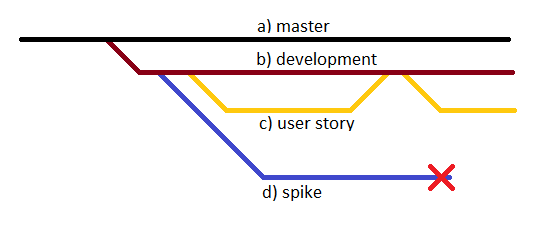
\includegraphics[width=0.9\textwidth]{git-XP-branches}
\caption{Git branching integrated into eXtreme Programming work flow}
\label{fig:gitXPbranches}
\end{figure}

The a)main branch  only contains a stable version of the program, everything is developed onto a b)development branch which may be unstable, when it stabilizes it merges back into the a)main branch. When a new user story is started it branches out from the b)development branch into a c)user story branch and is developed there, when the user story is complete and all of the tests pass it gets merged back to the b) development branch. There are also the occasional d)spike branches which are created for fast prototyping. They may branch out from anywhere and never make it back (they get thrown away).

Since my project is meant to be open-source I had no reservations about placing it on git-hub. The repository is located at: https://github.com/SuperIzzo/Vroom3D

\subsubsection{User stories}
An important element of the XP methodology are the user stories. My interpretation of this is an online sticky note board. I'm my own client and I don't have a constant workstation so it suits my needs. It could be accesses at http://www.stixy.com/guest/236395

\begin{figure}[htb]
\centering
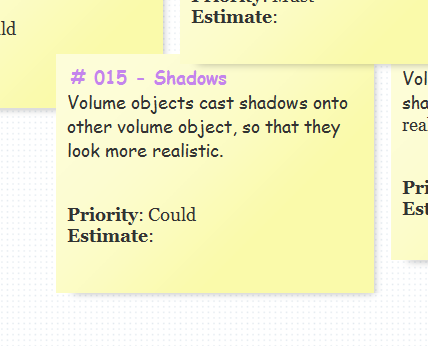
\includegraphics[width=0.3\textwidth]{user-story}
\caption{An example StixyBoard user story}
\label{fig:stixyUserStory}
\end{figure}

For priority I use the MoSCoW notation\cite{AgileModUserStories} (Must, Should, Could, Won't), to stay away from numbers (see \ref{fig:stixyUserStory}), I have not decided on estimation conventions yet, but it won't be numbers either.

I have written a few user stories but I need to complete a little crucial spike work \ref{sec:spikeWork}, before I can decide which way I want to move the project forward.

\FloatBarrier
\subsubsection{Project setup}
The project tree is structured as shown in \ref{fig:projectSetup}. The goals of this setup is to keep everything separate and independent, especially the IDE project files. At present it is a MSVC 2010 project, but I would like to make it a CMake project, so that it is easier to keep multi-platform project files consistency. I do not know CMake very well and this is currently in my wish list. 

The main product will be a library (in both static and dynamic form). Demo projects will produce executables, they will be in separate projects within the same solution. At present I have found the following third party libraries to be useful - UnitTest++\cite[UnitTest++], Eigen\cite[Eigen], SFML and Field3D\cite[Field3D] and have tried all of them except for Field3D.


\begin{SCfigure}
\centering
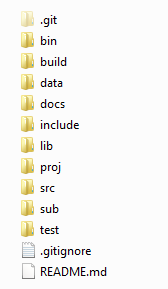
\includegraphics[width=0.35\textwidth]{project-structure}
\caption{Project tree structure. The project is set up using this 
tree structure. Source files and hidden API are located in the "src" directory,
public API headers go in the include folder. "test" is where all unit test files are located. "proj" contains project files. "sub" contains third party libraries. "docs" is where the documentation lives. Object files go into the "build" directory, while executables and dynamic libraries in "bin" and static libraries in "lib".
}
\label{fig:projectSetup}
\end{SCfigure}


\FloatBarrier
\subsection{Spike work}
\label{sec:spikeWork}

\begin{aquote}{Cyril Crassin\cite{CCrassinThesis}}
	``...there are three major issues to overcome before making detailed rendering of massive volumes
	a standard rendering primitive:
	\begin{itemize}
		\item How to store a pre-filtered voxel representation ?
		\item How to render it efficiently ?
		\item How to handle large amounts of voxel data ?
	\end{itemize}''
\end{aquote}

So far my focus has been on researching the different rendering methods and considering which one will be most suitable for use in interactive applications. With just some consideration on memory efficiency. Volume slicing is arguably faster\cite{AlgorithmComparison} because it is supported by hardware, but I have a personal bias towards ray-tracing, so I have been researching and experimenting with the two technologies.

Currently I only have an incomplete prototype of a ray-casting algorithm which I used to familiarize myself with the maths involved. \ref{fig:rayCube} illustrates my implementation of ray-cube clipping and local to voxel coordinate space conversion. I have also tried trilinear interpolation on colors.
\begin{figure}[htb]
\centering
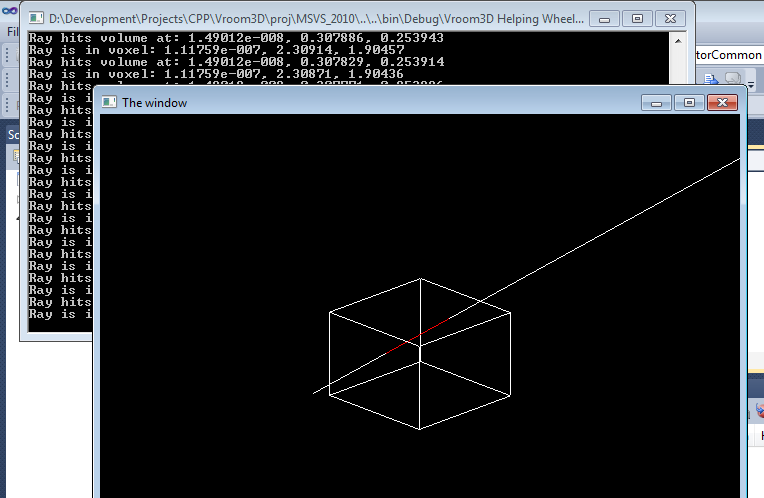
\includegraphics[width=0.4\textwidth]{ray-cube-intersection}
\caption{Ray-cube intersection using Cyrus-Beck line clipping}
\label{fig:rayCube}
\end{figure}
I am yet to load a volume object in memory and try rendering it using ray-tracing.

3D texture mapping is another thing I'm yet to try out. I have considered a few ways to reduce the memory demand of this method (which is its shortcoming), one of which is using static geometry composed of pre-computer orthogonal slices\cite{TextureMappingTut} rather than on-the-fly slices parallel to the camera. The benefits of this approach are that slices can be shrunk to enclose only the opaque part of the texture and discard the unnecessary pixel data, also the voxels between the slices no longer will need to reside in memory. It's drawback are that under certain angles the object will look distorted based on the slice density, also rendering order becomes an issue if the object is transparent as there will be crossing planes and because it is pre-calculated dynamic changes to the volume may be costly.
The optimisation in shown in \ref{fig:receedingPlates}  may be done however. We decrease the number of plates in relation to their dot product with the camera this way the more significant angle will be covered by the other sets of plates. Note that this way we can also easily determine the order of rendering, if the dot product is negative we render back to front (in object space) if the dot product is positive front to back.
\begin{figure}[htb]
\centering
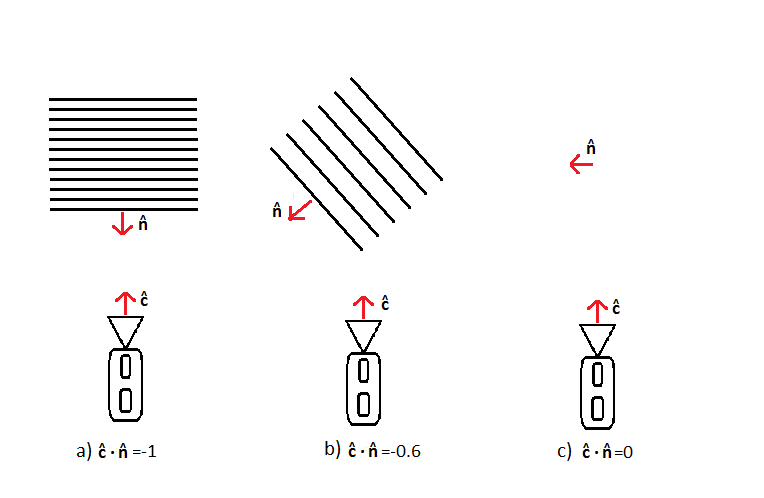
\includegraphics[width=0.4\textwidth]{receding-plates}
\caption{Receding plates}
\label{fig:receedingPlates}
\end{figure}




%==============================================================================
\section{Planning}
%==============================================================================

\subsection{Methodology}

The development methodology I chose is eXtreme Programming. The main reasons are because I was not aware with the requirements of the system I wanted to construct and I am still not fully aware of what the final version will look like, I have not been able to estimate the effort required and the amount of success I will achieve, so to reduce the risk I have to develop a flexible system that responds to changing requirements and uncertainties, which is what XP is good at. Of course I could not follow all of the practices strictly, because the methodology is based on teamwork, but I could follow most of them the full extend possible.
Meetings are replaced by brainstorming sessions with retrospectives, pair programming by code review, I am my own client, so I spare time to think about the goals of the system and write user stories.

Each iteration last one week and at the end of the iteration there will be a release.

\subsection{Demonstrations}

\subsubsection{Mid-project demonstration}
The first demonstration will be on the results of the spike work; it will possibly be a comparison of the two rendering methods and conclude my resolve on which technology I will use for the final deliverable I would have hopefully decided that before then and built on top of it. Ideally both technologies would be supported but that imposes huge architectural challenges as the data structures required for the optimal performance of each vary drastically.
The 

\subsubsection{End project demonstration}
The minimal set of features the final version will demonstrate are:
\begin{itemize}
	\item ability to render multiple volume object simultaneously
	\item render scenes at interactive frame rate (min 30 fps)
	\item ability to render maps of minimum 1024x1024x256 voxels (Voxlap\cite{Voxlap} standard)
	\item basic world, view, and volume object transformations
	\item ability to deal with transparent objects
	\item ability to destroy and deform portions of volume objects
	\item minimal resolution of 800x600
\end{itemize}

In addition the system may feature, dynamic lightning, shadows, bone animations, reflection and other.

\subsection{Milestones}
Here is a high level milestone map of deadlines.

\begin{description}
	\item[30 Nov, 2012]		Working ray-tracing prototype, able to render a single volume object. 	Working slice based prototype able to render the same volume object.
	\item[23 Dec, 2012]		Demo application able to render and transform several objects. Possibly dealt with transparency issues by then.
	\item[17 Feb, 2013]		Architecture in place, prototype has made it to the project.
	\item[03 Mar, 2013]		Solved memory issues.
	\item[17 Mar, 2013]		Solved performance issues.
	\item[31 Mar, 2013]		First draft of the final report.
	\item[21 Apr, 2013]		Final version of the final report and final version of the demo. 
\end{description}

Note that these are not final and only meant as a guide, the actual goal for each week will be determined at the start of the iteration. For instance a ray-tracer would have to deal with performance issues earlier, and a 3D texture map implementation will need to deal with memory first.

\nocite{*} % include everything from the bibliography, irrespective of whether it has been referenced.

% the following line is included so that the bibliography is also shown in the table of contents. There is the possibility that this is added to the previous page for the bibliography. To address this, a newline is added so that it appears on the first page for the bibliography. 
\newpage
\addcontentsline{toc}{section}{Annotated Bibliography} 

%
% example of including an annotated bibliography. The current style is an author date one. If you want to change, comment out the line and uncomment the subsequent line. You should also modify the packages included at the top (see the notes earlier in the file) and then trash your aux files and re-run. 
%\bibliographystyle{authordate2annot}
\bibliographystyle{IEEEannot}
\renewcommand{\refname}{Annotated Bibliography}  % if you put text into the final {} on this line, you will get an extra title, e.g. References. This isn't necessary for the outline project specification. 
\bibliography{mmp} % References file


\end{document}
